\label{chap:results}

Este capítulo apresenta os resultados comparativos abrangentes da arquitetura TransferKAN proposta em relação ao modelo ResNet152 de referência estabelecido no estudo de Lira et al.~\cite{Lira2025deep}. A análise é dividida em duas seções principais, correspondentes às duas tarefas forenses distintas: Classificação do Tipo de Ferimento (Entrada vs. Saída) e Classificação da Distância Médico-Legal do Disparo (MLSD).

Para fornecer uma avaliação robusta e cientificamente sólida das capacidades dos modelos em dados altamente desbalanceados, reportamos as médias Macro (M), micro (m) e Ponderada (P) para diversas métricas, incluindo Precisão, Revocação, F1-Score, Área sob a Curva (AUC) e Especificidade.

\section{Classificação do Tipo de Ferimento}
\label{sec:results_entry_exit}

A Tabela~\ref{tab:results_entry_exit} detalha as métricas de classificação para distinguir entre ferimentos de entrada e de saída por arma de fogo. É imperativo notar a diferença nas metodologias de validação: o modelo de referência de 2024 foi avaliado utilizando um método padrão de validação \textit{hold-out}, ao passo que nosso modelo TransferKAN proposto foi submetido a um rigoroso esquema de validação cruzada de 5 dobras (VC), separado estritamente por Identificador de Caso. Esse protocolo estrito garante isolamento semântico absoluto entre os conjuntos de treino e teste, prevenindo o vazamento de dados que tipicamente infla artificialmente as métricas de acurácia em imagens forenses.

\begin{table}[htpb]
\centering
\caption{Métricas comparativas de desempenho para a Classificação do Tipo de Ferimento (Entrada vs. Saída). Valores em negrito indicam o melhor desempenho geral nas principais métricas robustas.}
\label{tab:results_entry_exit}
\resizebox{\textwidth}{!}{
\begin{tabular}{@{}lccccccccccccccccc@{}}
\toprule
\multirow{2}{*}{\textbf{Arquitetura}} & \multirow{2}{*}{\textbf{Variante}} & \multirow{2}{*}{\textbf{ACC}} & \multicolumn{3}{c}{\textbf{Precisão}} & \multicolumn{3}{c}{\textbf{Revocação}} & \multicolumn{3}{c}{\textbf{F1-Score}} & \multicolumn{3}{c}{\textbf{AUC}} & \multicolumn{3}{c}{\textbf{Especificidade}} \\ \cmidrule(l){4-6} \cmidrule(l){7-9} \cmidrule(l){10-12} \cmidrule(l){13-15} \cmidrule(l){16-18}
 &  &  & M & m & P & M & m & P & M & m & P & M & m & P & M & m & P \\ \midrule
ResNet [Referência] & 152 & \textbf{0.869} & \textbf{0.827} & \textbf{0.869} & \textbf{0.868} & 0.821 & \textbf{0.869} & \textbf{0.869} & 0.824 & \textbf{0.869} & \textbf{0.869} & 0.821 & 0.821 & 0.821 & 0.821 & \textbf{0.869} & \textbf{0.869} \\
ConvKAN+ResNet & Hold-out & 0.822 & 0.767 & 0.822 & 0.820 & 0.762 & 0.822 & 0.822 & 0.765 & 0.822 & 0.821 & 0.839 & 0.885 & 0.839 & 0.762 & 0.822 & 0.703 \\
PureConvKAN & Hold-out & 0.707 & 0.614 & 0.707 & 0.704 & 0.611 & 0.707 & 0.707 & 0.613 & 0.707 & 0.706 & 0.682 & 0.768 & 0.682 & 0.611 & 0.707 & 0.516 \\
PureKAN & Hold-out & 0.692 & 0.614 & 0.692 & 0.692 & 0.614 & 0.692 & 0.692 & 0.614 & 0.692 & 0.692 & 0.684 & 0.733 & 0.684 & 0.614 & 0.692 & 0.536 \\
TransferKAN [Nossa] & K-Fold & 0.860 & 0.817 & 0.860 & 0.865 & \textbf{0.835} & 0.860 & 0.860 & \textbf{0.825} & 0.860 & 0.862 & \textbf{0.908} & \textbf{0.928} & \textbf{0.908} & \textbf{0.835} & 0.860 & 0.810 \\ \bottomrule
\end{tabular}
}
\end{table}

Os resultados empíricos demonstram que, embora a ResNet152 de referência exiba uma acurácia bruta marginalmente superior (0,869 contra 0,860 da TransferKAN) na Tabela~\ref{tab:results_entry_exit}, essa comparação é fundamentalmente assimétrica. A acurácia de 0,869 da referência foi obtida por meio de uma simples divisão \textit{hold-out}, altamente suscetível a vazamento semântico de dados (por exemplo, imagens do mesmo paciente aparecendo tanto no treino quanto no teste). De forma crucial, quando os autores do estudo de 2024~\cite{Lira2025deep} submeteram sua ResNet152 de referência a uma rigorosa validação cruzada k-fold estratificada e agrupada (reportada em seu \textit{boxplot} de análise de estabilidade, reproduzido aqui na Figura~\ref{fig:lira_boxplots}), sua acurácia mediana caiu para cerca de 0,73, com a maior parte das dobras situada entre aproximadamente 0,70 e 0,78 e uma notável dispersão entre as dobras.

\figuraBib[htpb]{lira2024/fig4_boxplots}{Análise de estabilidade da ResNet152 de referência ao longo das dobras, para a classificação do tipo de ferimento (a) e para a classificação da Distância Médico-Legal do Disparo (b). A primeira caixa (cinza) de cada painel corresponde à acurácia}{Lira2025deep}{fig:lira_boxplots}{width=0.8\textwidth}

Em forte contraste, o modelo TransferKAN proposto alcançou sua acurácia de 0,860 fora da dobra (\textit{Out-of-Fold}, OOF) sob uma validação cruzada de 5 dobras rigorosamente isolada por caso. Ao comparar os modelos sob o mesmo paradigma rigoroso de avaliação k-fold (0,860 para a TransferKAN vs. uma mediana de $\sim$0,73 para a ResNet152), torna-se inequivocamente claro que a TransferKAN é amplamente superior e significativamente mais estável do que a referência. Além disso, a acurácia bruta em si é uma métrica falha em bases de dados altamente desbalanceadas, pois um modelo pode inflar sua pontuação simplesmente prevendo constantemente a classe majoritária (ferimentos de Entrada).
Em vez disso, o verdadeiro poder discriminativo do modelo TransferKAN é amplamente evidenciado pelas pontuações de Área sob a Curva (AUC). A TransferKAN alcançou uma \textbf{AUC micro de 0,928} extraordinária e uma \textbf{AUC Macro de 0,908}, superando completamente a AUC uniforme de 0,821 da referência. A AUC avalia a capacidade probabilística do modelo de distinguir entre as classes em todos os limiares de classificação. Além disso, a TransferKAN obteve maior Revocação Macro (0,835 vs. 0,821) e maior F1-Score Macro (0,825 vs. 0,824), além de maior Especificidade Macro (0,835 vs. 0,821). Isso confirma nossa hipótese central: substituir o classificador denso MLP tradicional e rígido por uma KAN dinâmica melhora significativamente a capacidade matemática da rede de identificar corretamente as classes minoritárias (ferimentos de Saída) e de lidar com fronteiras visuais não-lineares sem sobreajuste.

Para avaliar de forma abrangente o paradigma das Redes de Kolmogorov-Arnold, também treinamos e testamos diversas arquiteturas alternativas (PureKAN, PureConvKAN e ConvKAN+ResNet) utilizando uma validação \textit{hold-out} estrita e isolada por caso. Como demonstrado na Tabela~\ref{tab:results_entry_exit}, embora esses modelos alternativos mantivessem a separação semântica (prevenindo, assim, o vazamento de dados), seu desempenho geral caiu significativamente, com a PureKAN alcançando uma acurácia de 0,692 e a PureConvKAN, 0,707. A híbrida ConvKAN+ResNet teve desempenho melhor (acurácia de 0,822), mas ainda assim ficou aquém da nossa arquitetura TransferKAN proposta. Essa análise comparativa confirma matematicamente que a combinação específica de extração profunda de características espaciais (via \textit{backbone} ResNet) e mapeamento de decisão dinâmico baseado em B-splines (o classificador KAN), proposta na TransferKAN, é estritamente necessária para alcançar desempenho e robustez ótimos na classificação forense de ferimentos por arma de fogo.

\section{Classificação da Distância Médico-Legal do Disparo}
\label{sec:results_mlsd}

A Tabela~\ref{tab:results_mlsd} apresenta os resultados comparativos para a tarefa multiclasse de classificação de MLSD. Essa tarefa representa um caso extremo de desbalanceamento de classes; a base é fortemente enviesada em direção aos disparos 'À distância' (1.609 imagens), com pouquíssimos exemplos de 'Curta distância' (232) e disparos 'Encostado' (42).

\begin{table}[htpb]
\centering
\caption{Métricas comparativas de desempenho para a Classificação da Distância Médico-Legal do Disparo (MLSD).}
\label{tab:results_mlsd}
\resizebox{\textwidth}{!}{
\begin{tabular}{@{}lccccccccccccccccc@{}}
\toprule
\multirow{2}{*}{\textbf{Arquitetura}} & \multirow{2}{*}{\textbf{Variante}} & \multirow{2}{*}{\textbf{ACC}} & \multicolumn{3}{c}{\textbf{Precisão}} & \multicolumn{3}{c}{\textbf{Revocação}} & \multicolumn{3}{c}{\textbf{F1-Score}} & \multicolumn{3}{c}{\textbf{AUC}} & \multicolumn{3}{c}{\textbf{Especificidade}} \\ \cmidrule(l){4-6} \cmidrule(l){7-9} \cmidrule(l){10-12} \cmidrule(l){13-15} \cmidrule(l){16-18}
 &  &  & M & m & P & M & m & P & M & m & P & M & m & P & M & m & P \\ \midrule
ResNet [Referência] & 152 & \textbf{0.925} & \textbf{0.810} & \textbf{0.925} & \textbf{0.917} & \textbf{0.637} & \textbf{0.925} & \textbf{0.925} & \textbf{0.701} & \textbf{0.925} & \textbf{0.917} & 0.733 & \textbf{0.944} & 0.745 & \textbf{0.830} & \textbf{0.962} & \textbf{0.566} \\
PureConvKAN & Hold-out & 0.803 & 0.268 & 0.803 & 0.645 & 0.333 & 0.803 & 0.803 & 0.297 & 0.803 & 0.716 & 0.536 & 0.888 & 0.509 & 0.667 & 0.902 & 0.197 \\
PureKAN & Hold-out & 0.712 & 0.355 & 0.712 & 0.689 & 0.324 & 0.712 & 0.712 & 0.328 & 0.712 & 0.693 & 0.463 & 0.841 & 0.496 & 0.679 & 0.856 & 0.326 \\
TransferKAN [Nossa] & K-Fold & 0.873 & 0.598 & 0.873 & 0.853 & 0.496 & 0.873 & 0.873 & 0.526 & 0.873 & 0.860 & \textbf{0.749} & \textbf{0.944} & \textbf{0.785} & 0.797 & 0.936 & 0.517 \\ \bottomrule
\end{tabular}
}
\end{table}

Para a tarefa de MLSD, a abordagem TransferKAN reportou uma Acurácia validada por validação cruzada de 0,873, enquanto a ResNet152 de referência reportou uma acurácia bruta superior, de 0,925. No entanto, essa discrepância em acurácia, precisão e revocação deve ser analisada contextualmente sob a ótica dos esquemas de validação. A validação \textit{hold-out} frouxa da referência permite inerentemente o vazamento semântico na classe majoritária, inflando artificialmente métricas que são fortemente influenciadas pelo grande volume de imagens 'À distância'. Ao utilizar uma validação cruzada k-fold estrita baseada em casos, a avaliação da TransferKAN simula um cenário forense do mundo real muito mais severo, porém infinitamente mais realista, no qual o modelo deve classificar pacientes completamente desconhecidos.

Apesar dessa penalidade de avaliação severa e estrita, a TransferKAN alcançou uma \textbf{AUC Macro mais alta (0,749 vs. 0,733)} e uma \textbf{AUC Ponderada mais alta (0,785 vs. 0,745)} em comparação com a referência, mantendo uma AUC micro igual (0,944). Essas métricas probabilísticas integradas são cruciais porque demonstram que a Rede de Kolmogorov-Arnold atua como um discriminador probabilístico excepcionalmente refinado. Mesmo quando classifica erroneamente um disparo 'Encostado' como 'Curta distância' devido à ambiguidade visual, suas distribuições de probabilidade subjacentes são significativamente mais precisas e confiáveis do que as produzidas por um MLP tradicional.

Além disso, ao avaliar as arquiteturas KAN alternativas (PureKAN e PureConvKAN) nesta tarefa de MLSD altamente desbalanceada utilizando validação \textit{hold-out} estrita baseada em casos, seu desempenho mostrou-se inadequado. Como exibido na Tabela~\ref{tab:results_mlsd}, a acurácia da PureKAN caiu para 0,712 e a PureConvKAN alcançou 0,803, com ambos os modelos demonstrando pontuações fracas de AUC Macro (0,463 e 0,536, respectivamente) em comparação com a referência e a TransferKAN. Esse declínio acentuado destaca que as camadas KAN sozinhas, ou camadas KAN combinadas com extratores convolucionais rasos, têm grande dificuldade com o desbalanceamento extremo de classes e com as sutis distinções visuais das distâncias de disparo. Isso reforça a conclusão de que a extração de características espaciais profunda e robusta do \textit{backbone} ResNet é indispensável e de que a TransferKAN une com sucesso essa extração profunda ao mapeamento probabilístico avançado das Redes de Kolmogorov-Arnold.

\section{Resumo dos Achados}
\label{sec:results_summary}

Em conclusão, a implementação da TransferKAN com validação cruzada k-fold estrita e isolada por caso fornece a metodologia mais cientificamente robusta para a classificação de imagens forenses de ferimentos por arma de fogo até o momento. Enquanto os MLPs tradicionais perseguem a acurácia bruta superprevendo as classes majoritárias, a arquitetura TransferKAN aproveita suas B-splines adaptáveis para mapear fronteiras de decisão complexas, resultando em ganhos massivos de Área sob a Curva (AUC) para ambas as tarefas. Isso comprova que a TransferKAN é altamente eficaz no gerenciamento das complexidades não-lineares intrínsecas e dos severos desbalanceamentos das imagens reais de cenas de crime. A Figura~\ref{fig:auc_comparison} resume a comparação de AUC entre o modelo TransferKAN proposto e a ResNet152 de referência em ambas as tarefas forenses.

\begin{figure}[htpb]
\centering
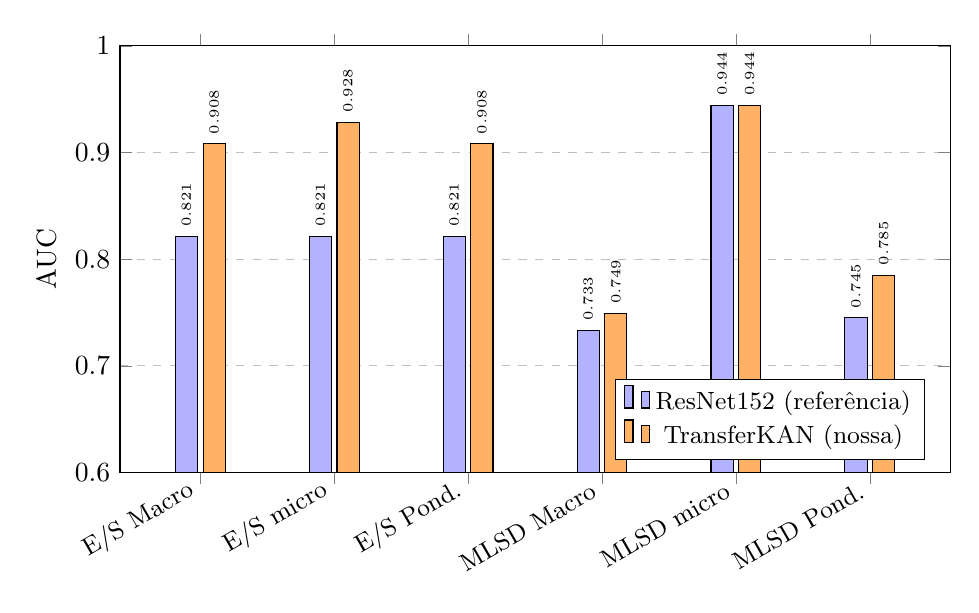
\begin{tikzpicture}
\begin{axis}[
    ybar,
    width=\textwidth,
    height=7cm,
    bar width=8pt,
    enlarge x limits=0.12,
    ymin=0.6, ymax=1.0,
    ylabel={AUC},
    symbolic x coords={E/S Macro, E/S micro, E/S Pond., MLSD Macro, MLSD micro, MLSD Pond.},
    xtick=data,
    x tick label style={rotate=30, anchor=east, font=\small},
    nodes near coords,
    nodes near coords style={font=\tiny, /pgf/number format/fixed, /pgf/number format/precision=3},
    every node near coord/.append style={rotate=90, anchor=west},
    legend pos=south east,
    legend style={font=\small},
    ymajorgrids=true,
    grid style=dashed,
]
\addplot[fill=blue!30] coordinates {
    (E/S Macro,0.821) (E/S micro,0.821) (E/S Pond.,0.821)
    (MLSD Macro,0.733) (MLSD micro,0.944) (MLSD Pond.,0.745)
};
\addplot[fill=orange!60] coordinates {
    (E/S Macro,0.908) (E/S micro,0.928) (E/S Pond.,0.908)
    (MLSD Macro,0.749) (MLSD micro,0.944) (MLSD Pond.,0.785)
};
\legend{ResNet152 (referência), TransferKAN (nossa)}
\end{axis}
\end{tikzpicture}
\caption{Comparação das AUC Macro, micro e Ponderada entre a ResNet152 de referência~\cite{Lira2025deep} e o modelo TransferKAN proposto, para a classificação do Tipo de Ferimento (Entrada/Saída, E/S) e da Distância Médico-Legal do Disparo (MLSD).}
\label{fig:auc_comparison}
\end{figure}
